\section{The \rnn{} Algorithm}%
\label{sec:neuralringer}


\subsection{Building the Rings}\label{ssec:rnn_for_online_and_eletrons}


The ATLAS calorimeters comprise rectangular cells in the
\etaphi plane for different layers in depth\footnote{Except for the forward calorimeters.}.
The calorimeter system covers the pseudorapidity\footnote{ATLAS uses a right-handed coordinate system with its origin at the nominal interaction point (IP) in the centre of the detector and the z-axis along the beam-pipe. The x-axis points from the IP to the centre of the LHC ring, and the y-axis points upward. Cylindrical coordinates (r, $\phi$) are used in the transverse plane, \phi being the azimuthal angle around the beam-pipe. The pseudorapidity is defined in terms of the polar angle $\theta$ as \eta = -$\ln{tan(\theta/2)}$. The angular distance $\Delta R$ is defined as $\Delta R = \sqrt{(\Delta\eta)^{2} + (\Delta\phi)^{2}}$ . Transverse momenta and energies are defined as $pT = p\sin\theta$ and $E_{T}$ = $E\sin\theta$, respectively.} range \(|\eta| < 4.9\)~\cite{PERF-2007-01}. 


Within the region $|\eta|< 3.2$, an electromagnetic calorimetry (ECAL) is provided by the high-granularity lead/Liquid-Argon (LAr) calorimeters contituted of barrel (EMB1,2,3) and endcap (EMEC1,2,3), with an additional thin LAr presampler (\ps) covering in barrel (PreSamplerB) and endcap (PreSamplerE), in order to correct for energy losses in material upstream of the calorimeters~\cite{LARG-2009-01,larg_tdr}. The Hadronic calorimetry (HCAL) is provided by the steel/scintillating-tile calorimeter (\tilecal)~\cite{TCAL-2017-01,tile_tdr}, constituted of three barrel structures (TileBar0, TileBar1 and TileBar2) within $|\eta| < 1.0$, three extended barrel structures (TileExt1,2,3) covering the region of $0.8<|\eta|< 1.7$ and two copper/LAr hadronic endcap calorimeters (HEC)
~\cite{cal_tdr} within $1.5<|\eta|< 3.2$ divided in four modules (HEC0,1,2,3). Transition regions between calorimeters are used to locate detector services and induce a sharing of showers between calorimeters that degrades energy measurements in those regions. Here, the transition from the barrel to the endcap is complemented by the intermediate tile calorimeter (ITC) composed by two modules (TileGap1,2,3) that are both attached on the face of the external barrel to estimate signal losses~\cite{cal_tdr}. The solid angle coverage is completed with forward
copper/LAr and tungsten/LAr calorimeter (FCal) modules optimised for electromagnetic (EM) and hadronic (HAD) measurements, respectively. The specified calorimeters
provide full azimuthal ($\phi$) coverage with a total of about 190,000 readout cells. 



The electromagnetic and hadronic calorimeters are segmented~\cite{PERF-2007-01}\footnote{The two
central layers in HCAL end-cap are summed to result in a single measurement.} longitudinally (i.e. in depth) into three sampling layers each where each layer has its own lateral ($\eta\times\phi$) granularity. Besides granularity, the amount of detector material in front of the detector in each sampling layer also varies with \abseta, leading to variations in the expected lateral and longitudinal profiles. Additionally, the expected
profile is also dependent on the physics object total energy. In the EM calorimeter, most of the EM shower energy is collected in the second layer (EM2), while the third layer (EM3) provides measurements of energy deposited in the shower tails. Although, it is important to mention that the first EM layer (EM1) plays an important role in the discrimination of electrons against $\pi^0$. The hadronic calorimeters, which surround the EM detectors, provide additional discrimination power through further energy measurements of possible EM shower tails, as well as rejection of events with activity of hadronic origin with three sampling layers (HAD1,2,3). 


As the algorithm was considered to operate online at \fastcalo{} stage in software, approximations were made. Specifically, the rectangular rings are constructed to match the grid layout of the calorimeter cells and the ring coverage is bounded by the RoI area. In addition, granularity changes from the cell sizes from different regions of the detector are neglected\footnote{The $\eta$ granularity used by the algorithm at EM1 layer is 0.003 for the entire eta range defined ($|\eta|<2.5$). However, the detector construction at this layer cover the region of $0<|\eta|<2.37$ and has different granularities in $\eta$: starts with 0.003 at $0<|\eta|<1.81$; 0.004 at $1.81<|\eta|<2.01$ and 0.006 at $2.01<|\eta|<2.37$.} in order to employ a grid-like algorithm.


Here, the algorithm RoI covers a
region of the calorimeter, centered in the L1 provided RoI, of
$0.4\times0.4$ in the $\eta\times\phi$ plane. The algorithm
starts on the second EM sampling layer (EM2)\footnote{This convention is used for all sampling layers, thus HAD1 stands for the first hadronic layer, HAD2 the second hadronic layer etc.}, where position given in $\eta\times\phi$ plane of the cell with highest $E_T$ on the algorithm RoI is taken as the center of the cascade interaction in the calorimeter. The initial seed cell position is propagated to other calorimeter layers in order to define the axis of the rings in that layer. Then, for each layer, the algorithm refines the seed position searching for most energetic cell inside of the window centred on the EM2 initial seed and the energy deposition of an incoming particle is extracted by building concentric rings of cells, or simply ``rings''. 

\begin{figure}[h!t]
	\centering
	\begin{center}
		\begin{subfigure}[c]{.95\textwidth}
			\centering
			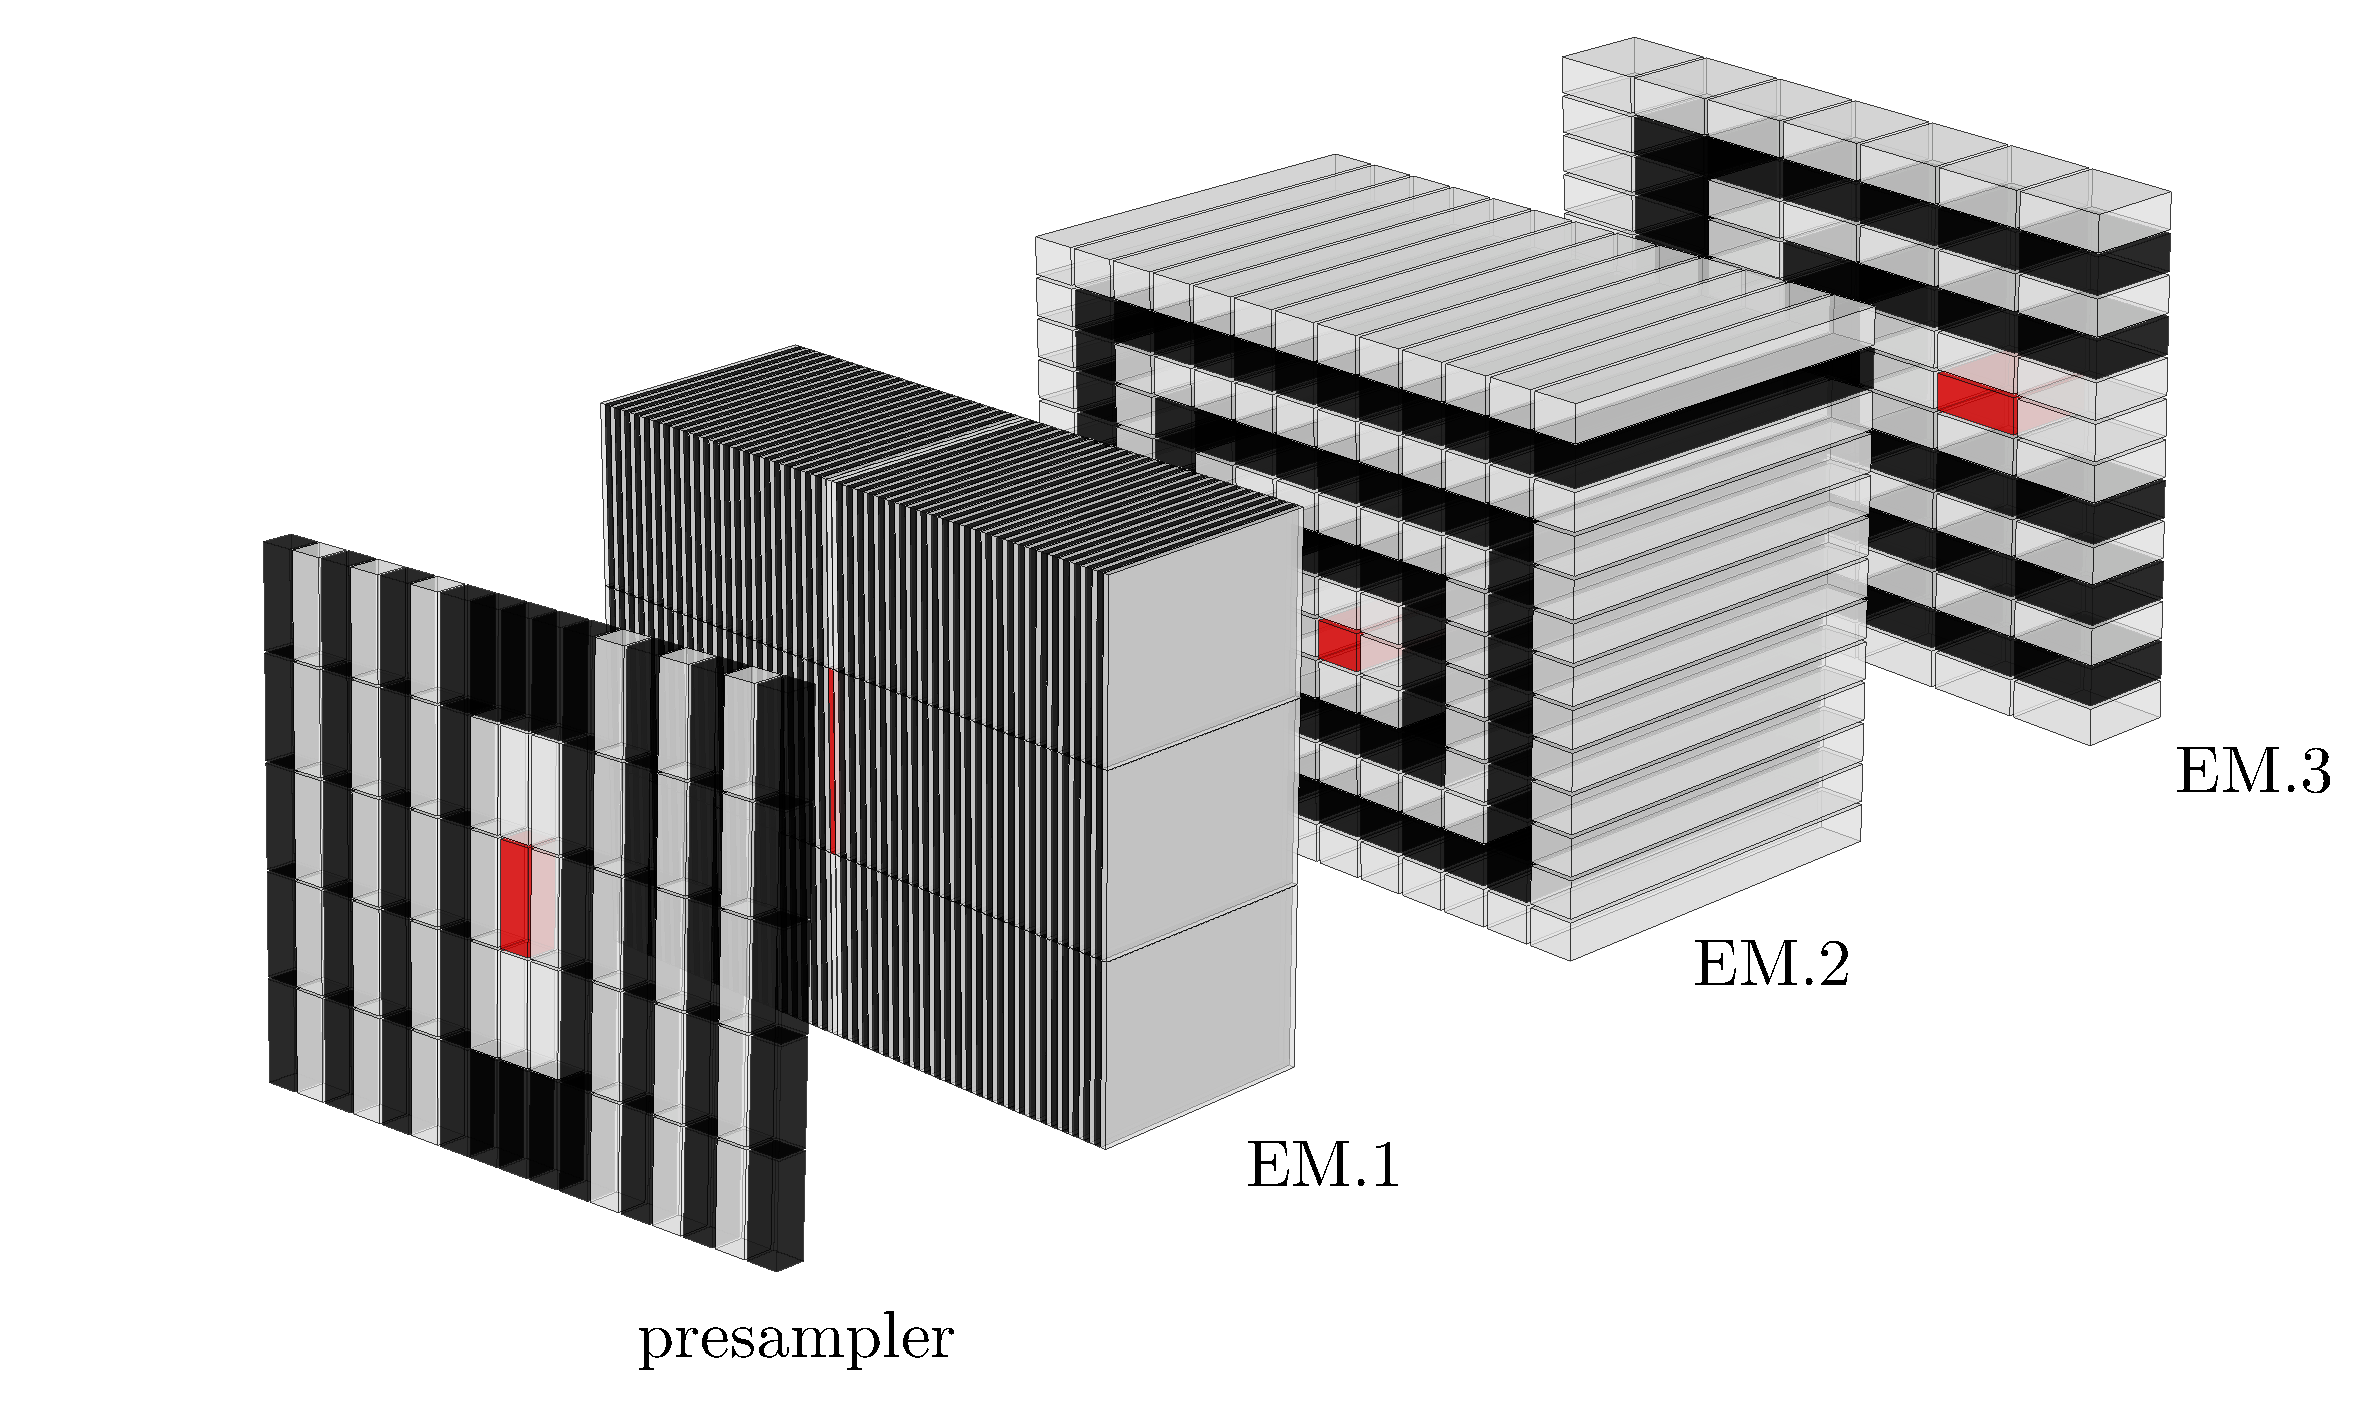
\includegraphics[width=\textwidth]{sections/02_ringer/figures/ATLAS_EM_Layers_v5.pdf}
			\caption{Eletromagnetic calorimeter cells within the ringer reconstruction window.}
		\end{subfigure} \\
		\begin{subfigure}[c]{.95\textwidth}
			\centering
			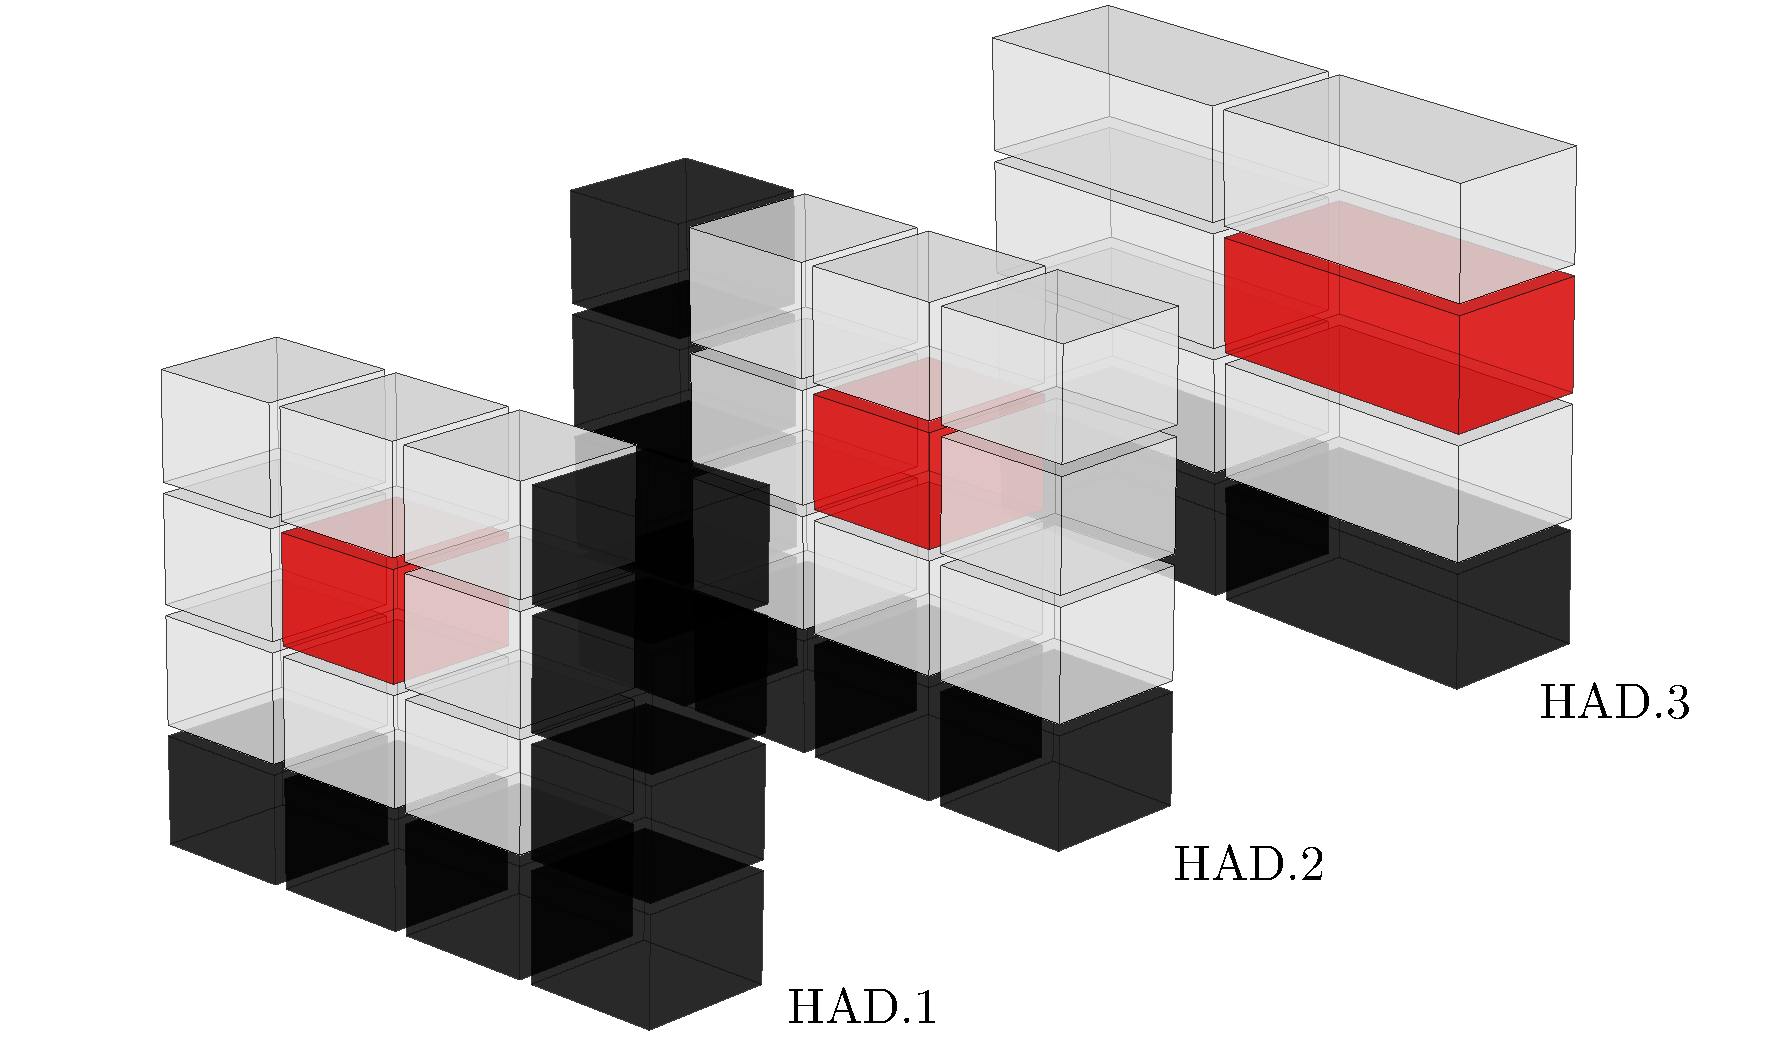
\includegraphics[width=\textwidth]{sections/02_ringer/figures/ATLAS_HAD_Layers_v5.pdf}
			\caption{Hadronic calorimeter cells within the ringer reconstruction window.}
		\end{subfigure}
	\end{center}
	\caption{\label{fig:calo_rings}
		Sketch to illustrate the ring-shaped energy description.
		The most energetic cell is in red, while the consecutive neighbouring rings are represented by alternating gray and black cells.
	}
\end{figure}

The refined seed ($c_{hot,l}$) will be used as starting point to build the rings. A ring $R_{n,l}$ contains all cells in calorimeter layer $l$ which are $n$ cells from the refined seed (See \figurename~\ref{fig:calo_rings} for an illustration of the parameters). Formally,


\begin{equation}
%\label{eq:ring_idx}
R_{n,l} = \left\{c_{n,l} \mid n = \left\lfloor \max{\left( 
\frac{| \eta_{i,l} - \eta_{hot,l} |}{h_{\eta,l}}, 
\frac{| \phi_{i,l} - \phi_{hot,l} |}{h_{\phi,l}} 
\right)} \right\rceil, 
\forall c_{i,l} \in
\Theta_{RoI,l}
\right\},
\end{equation}



\noindent where (analogous to $\phi$ when suitable): $\eta_{i,l}$
and $\eta_{hot,l}$ are respectively the $c_{i,l}$ and $c_{hot,l}$
cells position in $\eta$; $h_{\eta,l}$ is the $l^{th}$ layer cell size in $\eta$; $\Theta_{RoI,l}$ is the set of cells
in the $l^{th}$ layer which are within the Ringer RoI and $\lfloor \cdot \rceil$ is the \textit{round} function.
\tablename~\ref{tab:ring_alg_parameters} shows the number of rings computed at each layer and the respective granularity.


\begin{table}[ht!]
\centering
\caption{Nomenclature defining the \rnn{} algorithm layers and sections, as well as the respective parameters employed and calorimeter sampling layers from which the cells are extracted. The \rnn{} algorithm parameters are dependent on the ringer layer $l$ and independent on \eta{} and \et{} during Run~2. The parameters are the ring size in \eta{} ($h_{\eta,l}$), $\phi$ ($h_{\phi,l}$) and the number of rings to be computed in each layer ($\text{N}_l$).
}%
\label{tab:ring_alg_parameters}
\resizebox{.8\textwidth}{!}{%
\begin{tabular}{lc|ccc|ccc}
\hline
\hline
\multicolumn{2}{c|}{Ringer} & \multicolumn{3}{c|}{Calorimeter Sampling} & 
\multicolumn{3}{c}{Parameters} \\
\hline
Section & Layer ($l$) & Barrel & \itc & End-cap & $h_{\etaa,l}$ & $h_{\phii,l}$ & $N_l$ \\
\hline
\hline
\multirow{4}*{EM} & \ps &  \presamplerb & & \presamplere & 0.025 & 0.1 & 8 \\
\cline{2-5}
& \emi & \emb{1} &  & \emec{1} & 0.003 & 0.1 & 64  \\
\cline{3-5}
& \emii & \emb{2} &  & \emec{2} & 0.025 & 0.025 & 8 \\
\cline{3-5}
& \emiii & \emb{3} &  & \emec{3} & 0.050 & 0.025 & 8 \\
\cline{1-5}
\multirow{6}*{HAD} & \multirow{2}*{\hadi} & \tilebar{0} &
\multirow{2}*{\tilegap{3}} & \multirow{2}*{\hec{0}} & \multirow{2}*{0.1} & \multirow{2}*{0.1} & \multirow{2}*{4} \\
&                     & \tileext{0} &                               &                           \\
\cline{3-5}
& \multirow{2}*{\hadii} & \tilebar{1} & \multirow{2}*{\tilegap{1}} & \hec{1}       & \multirow{2}*{0.1} & \multirow{2}*{0.1} & \multirow{2}*{4} \\
&                   & \tileext{1} &              & \hec{2}  \\
\cline{3-5}
& \multirow{2}*{\hadiii} & \tilebar{2} & \multirow{2}*{\tilegap{2}} & \multirow{2}*{\hec{3}} & \multirow{2}*{0.2} & \multirow{2}*{0.1} & \multirow{2}*{4} \\
&                     & \tileext{2} &                &             \\
\hline
\hline
\end{tabular}
}
\end{table}

The sum of the transverse energies of cells $c_{n,l}$ in the ring $R_{n,l}$ form a vector of discriminating quantities. They are ordered outwards and from the innermost layer of the calorimeter and provide the ring-shaped information of the RoI.




The ring building process resulting in 100 rings in total across all calorimeter layers. Thereby, a dimensionality reduction is provided by compacting the typical input space dimensionality of approximately 1000--1200 cells per ROI into the above-mentioned 100 rings through the usage of EM shower physics knowledge: the rings can keep a complete description of the symmetric lateral and longitudinal information. However, the algorithm only approximates this concept in order to meet the online operation requirements and avoid further manipulation of the instrumented information. 
Figure~\ref{fig:rings_profile} shows the ring-shaped mean profile differences between electrons and jet particles. 



\begin{figure}[!ht]
  \centering
  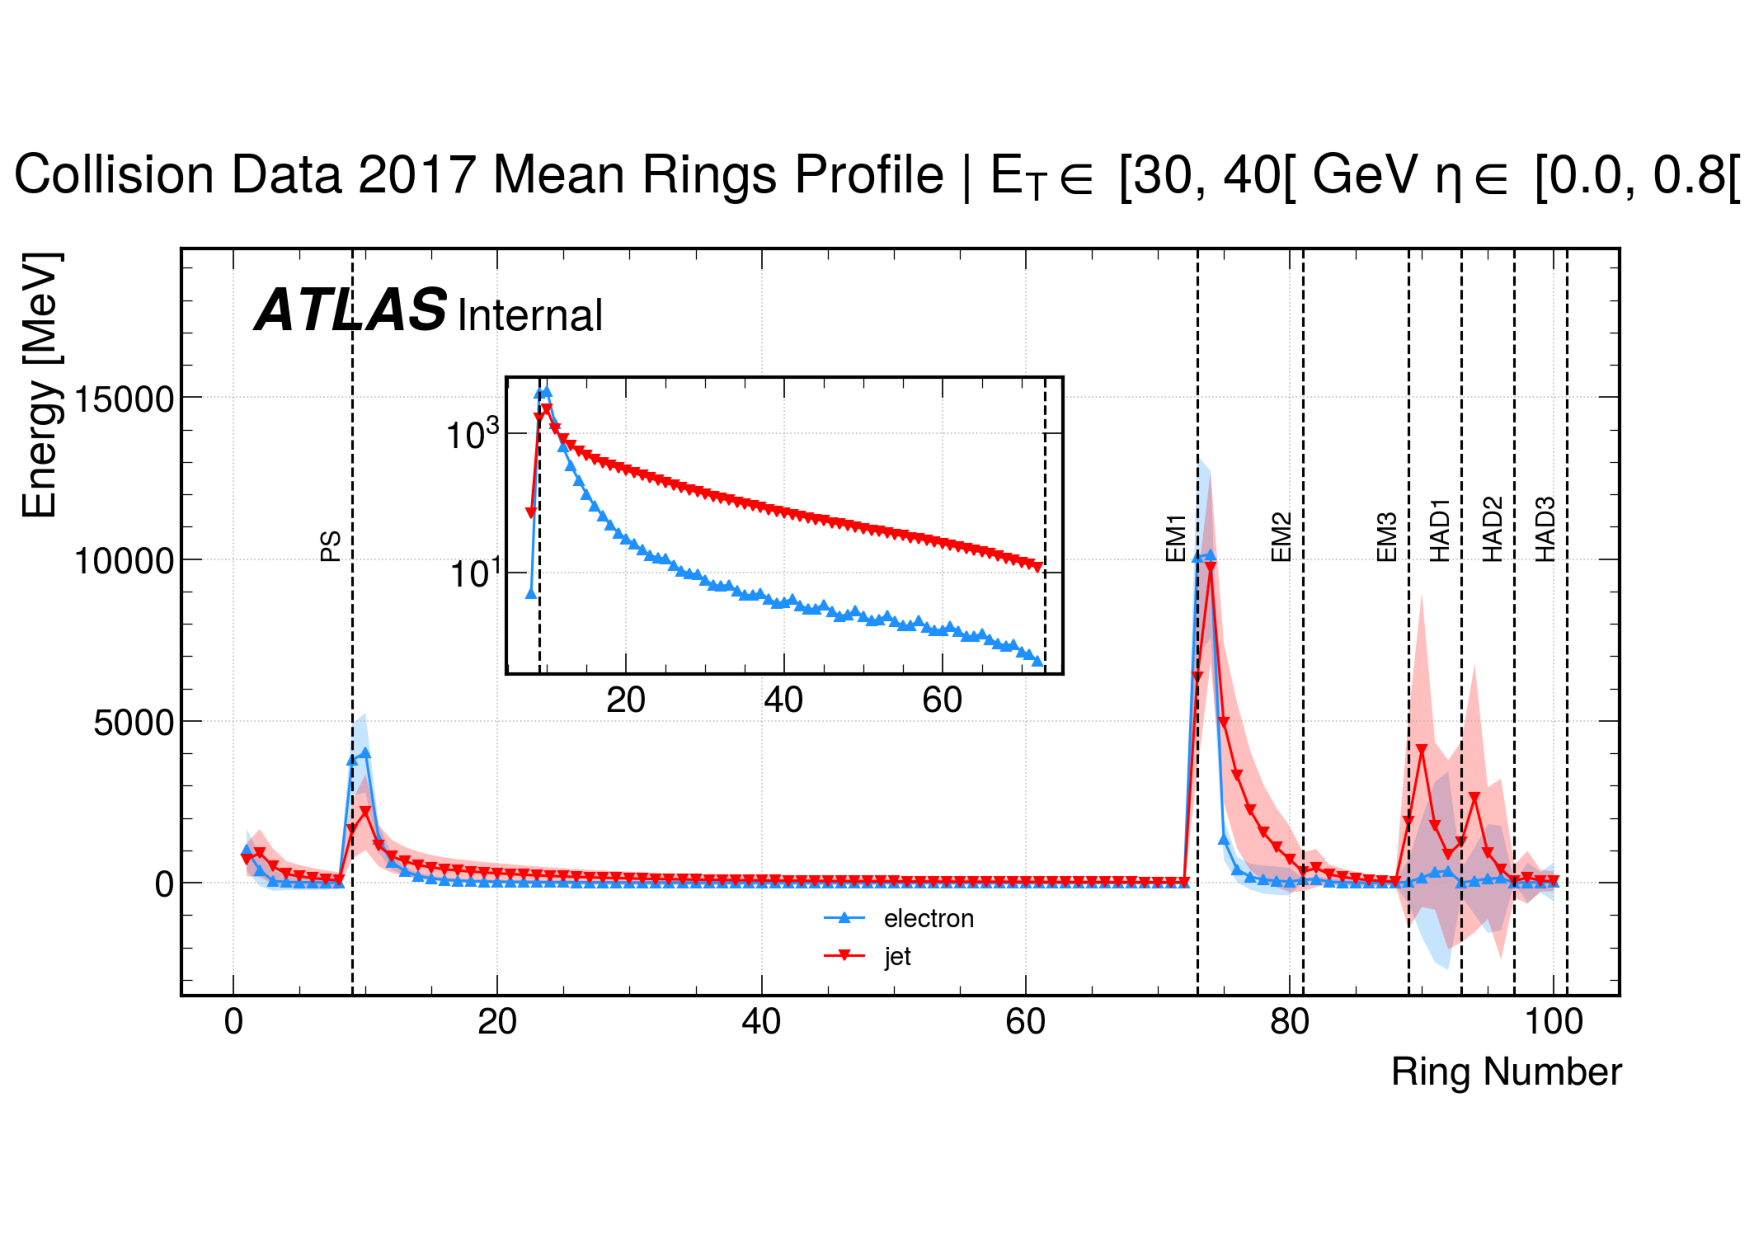
\includegraphics[width=0.7\textwidth]{sections/02_ringer/figures/reco_steps/data17_zee_mean_rings_profiles_et2_eta0.pdf}
  \caption{Average ring profile from collision data at $30 \leq E_T < 40$ GeV and $0.0 \leq \eta < 0.8$ for each layer of the calorimeter. The embedded profile shows the EM1 layer ring energies in a logarithmic scale. Here, it is possible to observe that most part of the energy for the electrons is absorbed by the eletromagnetic layers. For the jets, the opposite is observed and most of the energy is absorbed by the hadronic layers.}
  \label{fig:rings_profile}
\end{figure}

\subsubsection{Ring Sums as Discriminant Variables}

The current strategy concatenates all rings in a single vector of 100
variables. An absolute normalization using the total RoI energy is applied to normalize the variables. 
This procedure was initially proposed and examined by~\cite{1995_seixas_ringer}, as a way of preserving the shower energy profile in fractions of the total energy. 
The absolute value is used to avoid reflecting the values along the axis due to negative noise accumulation, a behavior which would impact the physics
representation of the normalized values and require a more complex decision
boundary:

\begin{equation}
  r^\prime_{k} = \frac{r_{k}}{| \sum\limits_{i=1}^{100} r_i
  |}, \;\;\;
    \forall \; k\in\{1,\dots,100\}.
\label{eq:ring_norm}
\end{equation}

Where $r_k$ or $r_i$ is the transverse energy of the ring with index $k$ or $i$ and $r^\prime_{k}$ is the normalized ring value with index $k$. It is specially valuable for its simplicity as it uses of a non parametric approach, and for allowing easy interpretation of the shower profile.



\subsection{Motivation for a Set of Neural Networks}\label{ssec:nn_set}

The normalized concatenated ring vector feeds a set of MLPs. A single
model is drawn from the set for operation based on the nearest region on the \eteta space for which it was designed.

In regards to calorimetry, the usage of a set with specific models per phase space region allows to mitigate fluctuations in the variable profiles
due to the detector response and energy differences of the showers.
A large contribution comes from granularity changes, which are discrete
in the phase space. Other important factors 
influencing such profiles are the
amount of the material as a function of \abseta{} and the dependence of
underlying processes in the shower development with respect to the incoming
particle energy. Although these alterations are mostly continuous, it is also
possible to approach the problem using space discretization.



At the hardware resource level, splitting the training into multiple small models to accommodate inhomogeneity of the detector response speeds up the training cycle and allows to handle data in memory, since only a small portion of the data is used to train that specific model. Limiting the memory requirement for tuning the models is particularly interesting in order to benefit from low-memory processing nodes, which were predominantly available in 
WLCG~\cite{2015_lcg_tdr} during our developments.\@ In addition, the decomposition of the problem can also lead to a reduction of the training time~\cite{Polikar2006}, as observed heuristically\footnote{
  When using NVIDIA RTX 2080Ti in tensorflow 1.14 and a minibatch size of 1024, a MLP with single hidden layer, a substantial increase in the runtime (from 4 to 41 seconds per epoch) with respect to the set version was observed.} 
when comparing the tuning time of the set to a single model. 
Regarding the operation, the proposed set only requires the choice of a
single model to operate instead of a more often committee machine approaches
that require the computation of different models in parallel with a fusion
method~\cite{zhou_ensemble}.  Therefore, the chosen set configuration adds
minimal overhead in terms of trigger latency. Similarly, the choice was to
operate with low-complexity models, a single hidden layer with few neurons, to obtain a competitive method with respect to the cut-based approach, in terms of processing speed.



\subsection{Training and Decision Making for 2017 and 2018 Operation}%
\label{sec:tuning}

\subsubsection{Data sets and Event Selection}%
\label{ssec:dataset}

The training procedure for 2017 operation was built with samples of 2015 simulated $Z\rightarrow ee$ decay, selected by the $Z\rightarrow ee$ \TnP method\cite{aad2020performance}, and background. For simulated background samples, a filter was applied to enrich with particles produced in the hard scatter with a summed transverse energy exceeding 17 GeV in a region of $\Delta\eta\times\Delta\phi=0.1\times0.1$. During 2016 data taking, the pile-up reached was 40 interactions per bunch crossing.
Here, both simulated samples include a pile-up of 60 interactions in average, per bunch crossing, which had never been seen before in collision data until the end of 2017, when the observed peek pile-up exceeded 60. Recently, in 2023, the highest level of pile-up observed exceeded 60 again.

After the training stage, thresholds on the discriminating score must be determined for selection of good electron candidates. To set the correct value without causing any inefficiency in the end of the HLT in collision data, the probe electrons, selected by $Z\rightarrow ee$ \TnP method and approved by the tightest offline available criteria, from full \textit{pp} data recorded by ATLAS in 2016 with LHC operating at a centre-of-mass energy of $\sqrt{s}=13\text{ TeV}$ was used. For background, objects rejected by the $Z\rightarrow ee$ \TnP method, that does not belong to any tag-probe electron pair, and reproved by the loosest offline available criteria were used. For the 2018 operation, the purely data-driven strategy was used, selecting events from the 2017 recorded collision data to train the models and adjust all thresholds. The tuning and analysis performed on collision data recorded have their quality ensured by the data quality procedure. 


\subsubsection{Training and Decision Making}%

The 2017 procedure derived the MLP models with simulated samples and defined the discriminant cut using 2016 collision data, targeting a signal efficiency similar to that of the cut-based trigger. The training procedure and decision making processes are the same for all phase space regions. For the \rnn{}, each MLP is an expert model for a single phase space region, containing its own topology and parameters.

The model parameters have been optimized using events selected on simulation datasets (Section~\ref{ssec:dataset}). 
The structure is a fully-connected single hidden layer, which may contain from 5 to 20 hidden units, an input layer with 100 inputs, one for each ring, and an output layer with a single neuron. 
The activation functions for both hidden and output neurons are the hyperbolic tangent, which has been often used in MLP designs~\cite{haykin_2008}. 

To assess the statistical fluctuations of the efficiency measurements, the stratified k-fold ($k=10$) cross-validation method~\cite{haykin_2008} was used at the price of increased computational cost by repeating training and testing procedures on different randomly chosen subsets. 
The stratified k-fold is among the most common cross-validation techniques and consists of partitioning the dataset in k disjoint subsets, each model tested with the $i$th subset and trained with the remaining ones. The dataset stratification follows the empirical order of the event selection, in order to allow straightforward job parallelization, i.e.\ random permutation is not employed. 

For each cross-validation sort and working point, 100 networks, initiated as from~\cite{initnw}, are optimized by back-propagating the Mean Squared Error (MSE) through the RPROP algorithm~\cite{rprop}. This repeated model initialization aims at avoiding poor sub-optimal solutions due to the usage of gradient-based algorithms.
For each training procedure, only three models out of the 100 are retained: two for retrieving the best efficiency when fixing the sensitivity or false positive probabilities to the baseline \fastcalo{} efficiency and another resulting in the \spmax{}\footnote{The SP value is defined as $\sqrt{\sqrt{P_D(1-F_A)}\cdot\frac{P_D + (1-F_A)}{2}}$ where $P_D$ is the signal detection probability (or sensitivity) and $F_A$ is the probability of a fake signal (false positive).} value. Early stopping~\cite{haykin_2008} is employed to avoid model over-training. The selection of the optimal iteration and operating model is based on an heuristic approach (multi-stop)~\cite{Goodfellow2016}.


Computational resources were used to tune 1.3~M shallow-learning neural networks, which resulted in a set of \SI{20}{MLPs} (five in \et{} $\times$ four in \abseta{}) for each one of the four working points used by electron triggers in the HLT. 
Here, the first training strategy considered only four regions in $|\eta|$ ($0.0\rightarrow 0.8\rightarrow1.37\rightarrow2.5$) and five region in $E_T$ ($15\rightarrow 20\rightarrow 30\rightarrow 40\rightarrow 50\rightarrow\infty$).
Except for few exceptions, the models in the set employed 5 neurons in the hidden layer. 

After the training stage, the decision is taken by applying a threshold in the one-dimensional output node of each expert MLP. 
Inspired by the HLT likelihood algorithm, the threshold applied for \rnn is also computed as a linear function of \avgmu{}.
However, a non-linear behavior was observed near the asymptote of the output activation function (See Figure~\ref{fig:nn_correction_with_tansig}), which occurred for the medium and tight operation points. Heuristically, it was 
observed that this behaviour can be avoided when replacing the hyperbolic tangent activation function from the output neuron by a linear function (Figure~\ref{fig:nn_correction_without_tansig}) for operation, after the training stage is completed.
This strategy provides a linear behavior of the targeted signal efficiency with respect to the online pile-up estimator. 
To account for Monte Carlo and collision data mis-modeling (See Figure~\ref{fig:nn_mc15_vs_data16}), the parameters of the linear threshold correction were derived using 2016 collision data and upper-bounded\footnote{in case of pile-up higher than upper-bound, the corrected threshold value is fixed.} by $\avgmu=40$ collisions. 


\begin{figure}[h!tb]
  \begin{center}
  %\hspace{0.01\textwidth}
  \begin{subfigure}[c]{.48\textwidth}
  \centering
  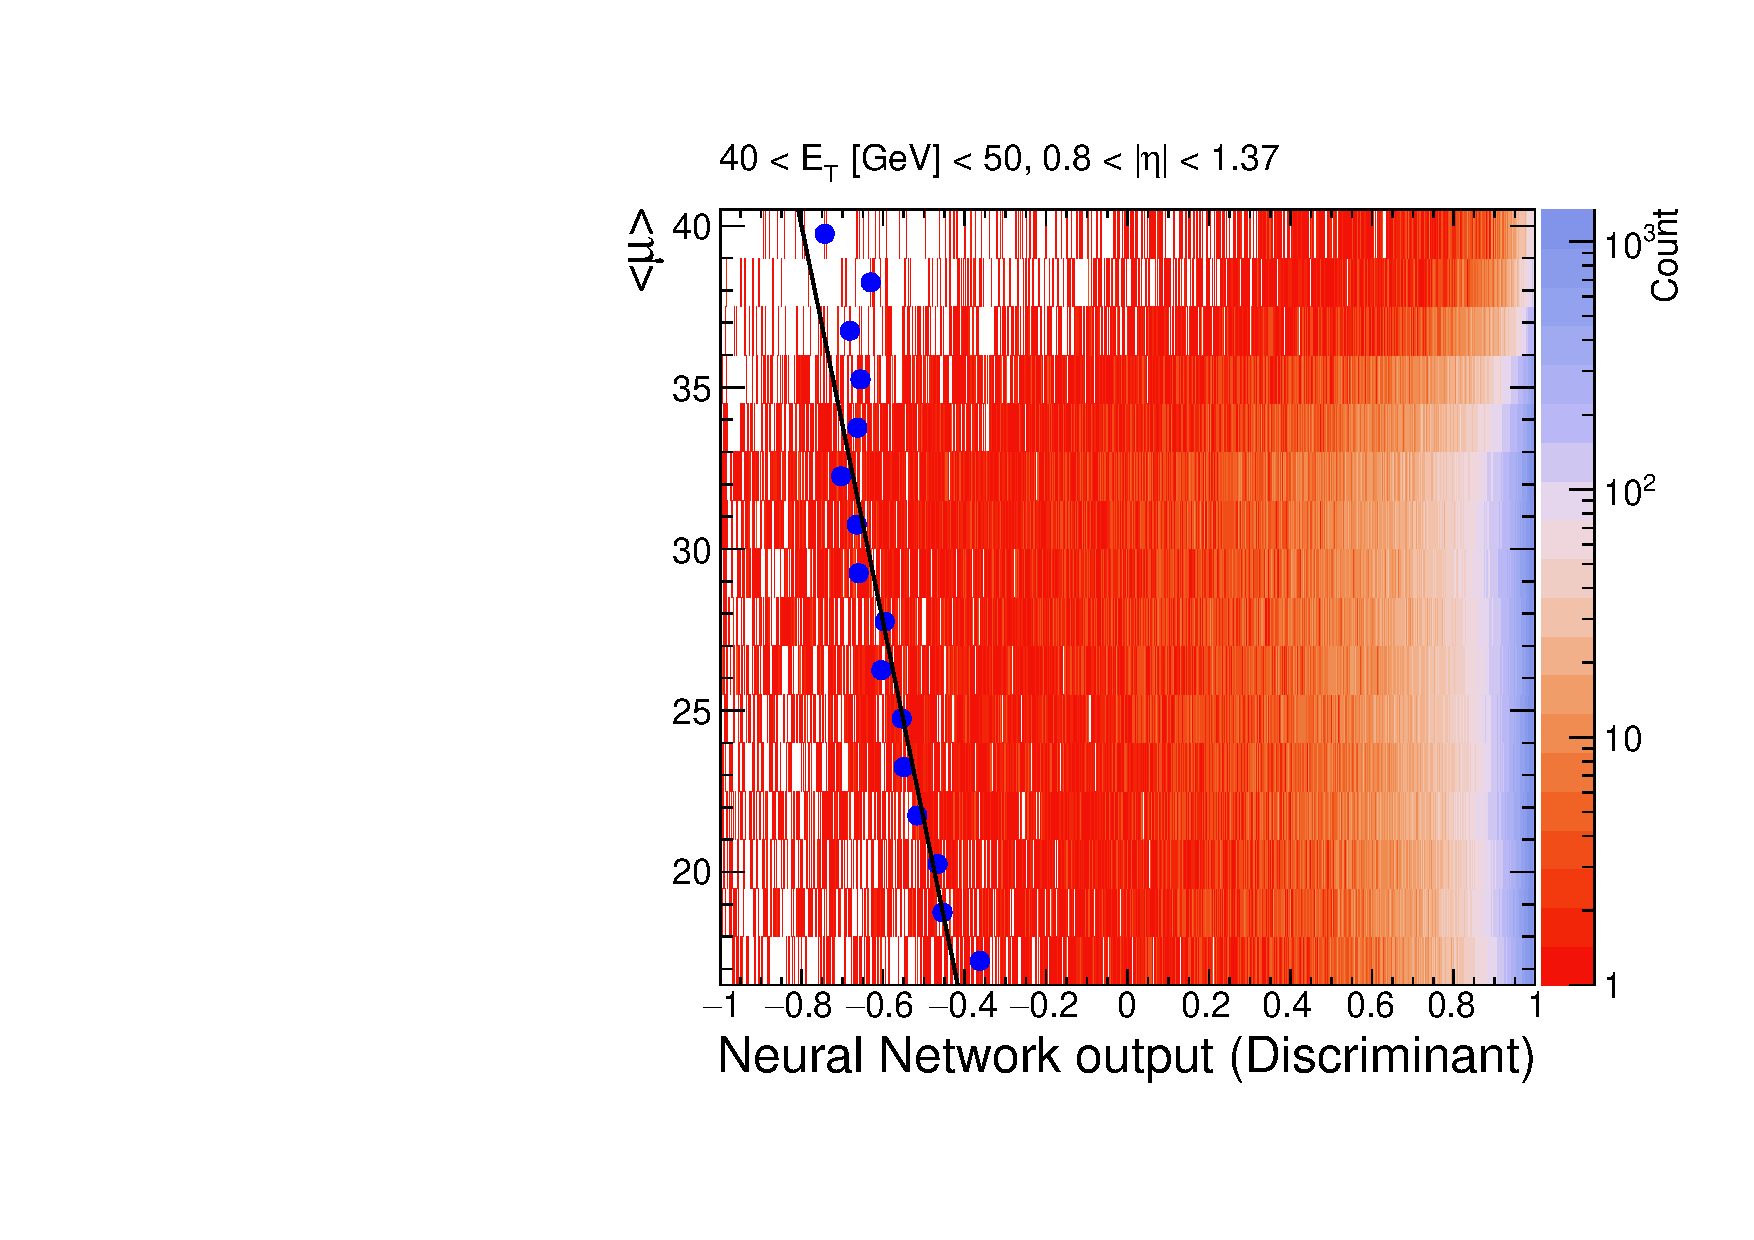
\includegraphics[width=\textwidth]{sections/02_ringer/figures/th2_signal_tight_cutbased_et3_eta1_with_tansig.pdf}
  \caption{MLP output with hyperbolic tangent as activation function in the output neuron w.r.t pile-up.}
  \label{fig:nn_correction_with_tansig}
  \end{subfigure}
  \hfill
  \begin{subfigure}[c]{.48\textwidth}
  \centering
  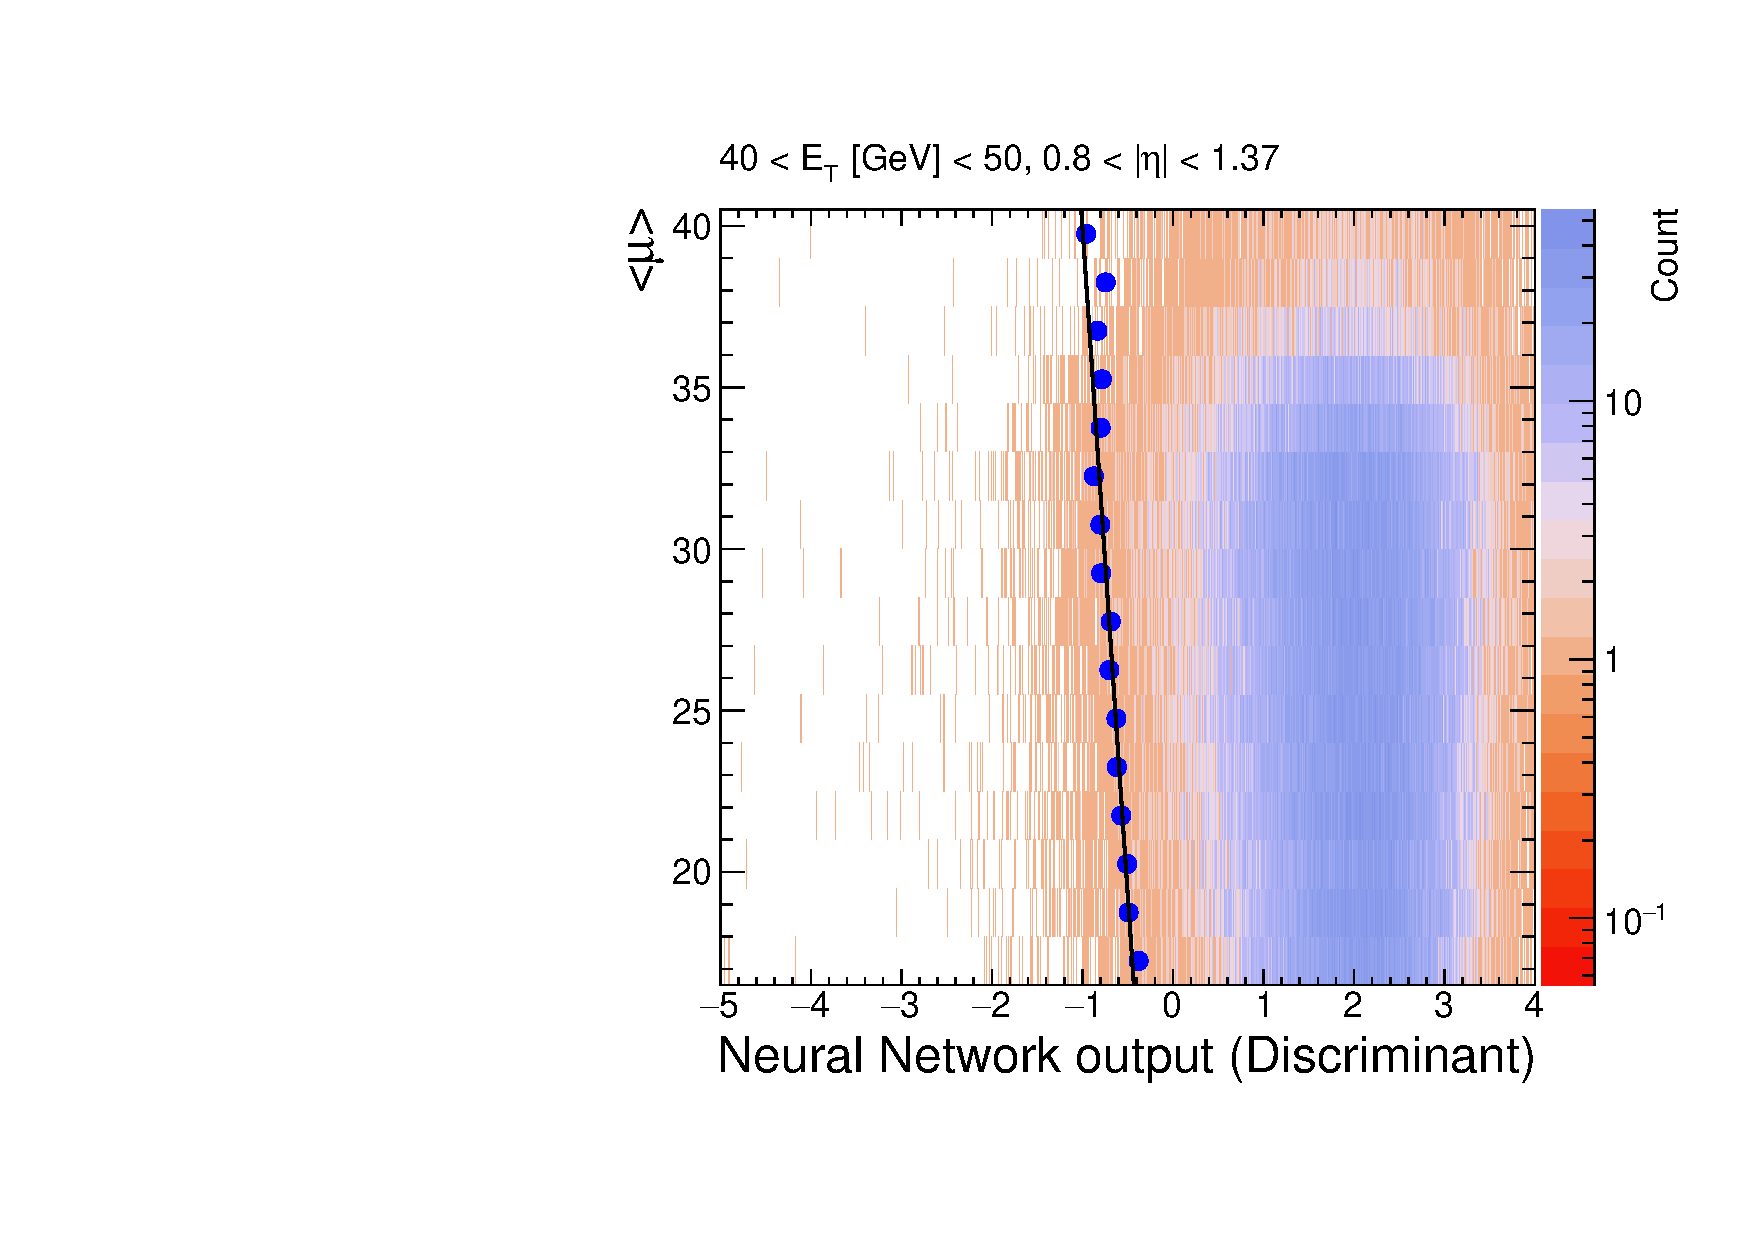
\includegraphics[width=\textwidth]{sections/02_ringer/figures/th2_signal_tight_cutbased_et3_eta1_without_tansig.pdf}
  \caption{MLP output with linear activation as activation function in the output neuron w.r.t pile-up.}
  \label{fig:nn_correction_without_tansig}
  \end{subfigure}
  %\hfill
  \caption{
    \rnn output as a function of \avgmu{} for $Z\rightarrow ee$ probes in 
    2016 collision data selected using the training criteria.
    The computed threshold per \avgmu{} unit for achieving the target 
    efficiency is shown in blue full circle. The black line is a linear fit of the thresholds.
    The output space is computed using the trained model without modifications 
    in (a), while in (b) the activation function from the output neuron is replaced by a linear function.
  }%
  \end{center}
\end{figure}

\begin{figure}[!ht]
  \centering
  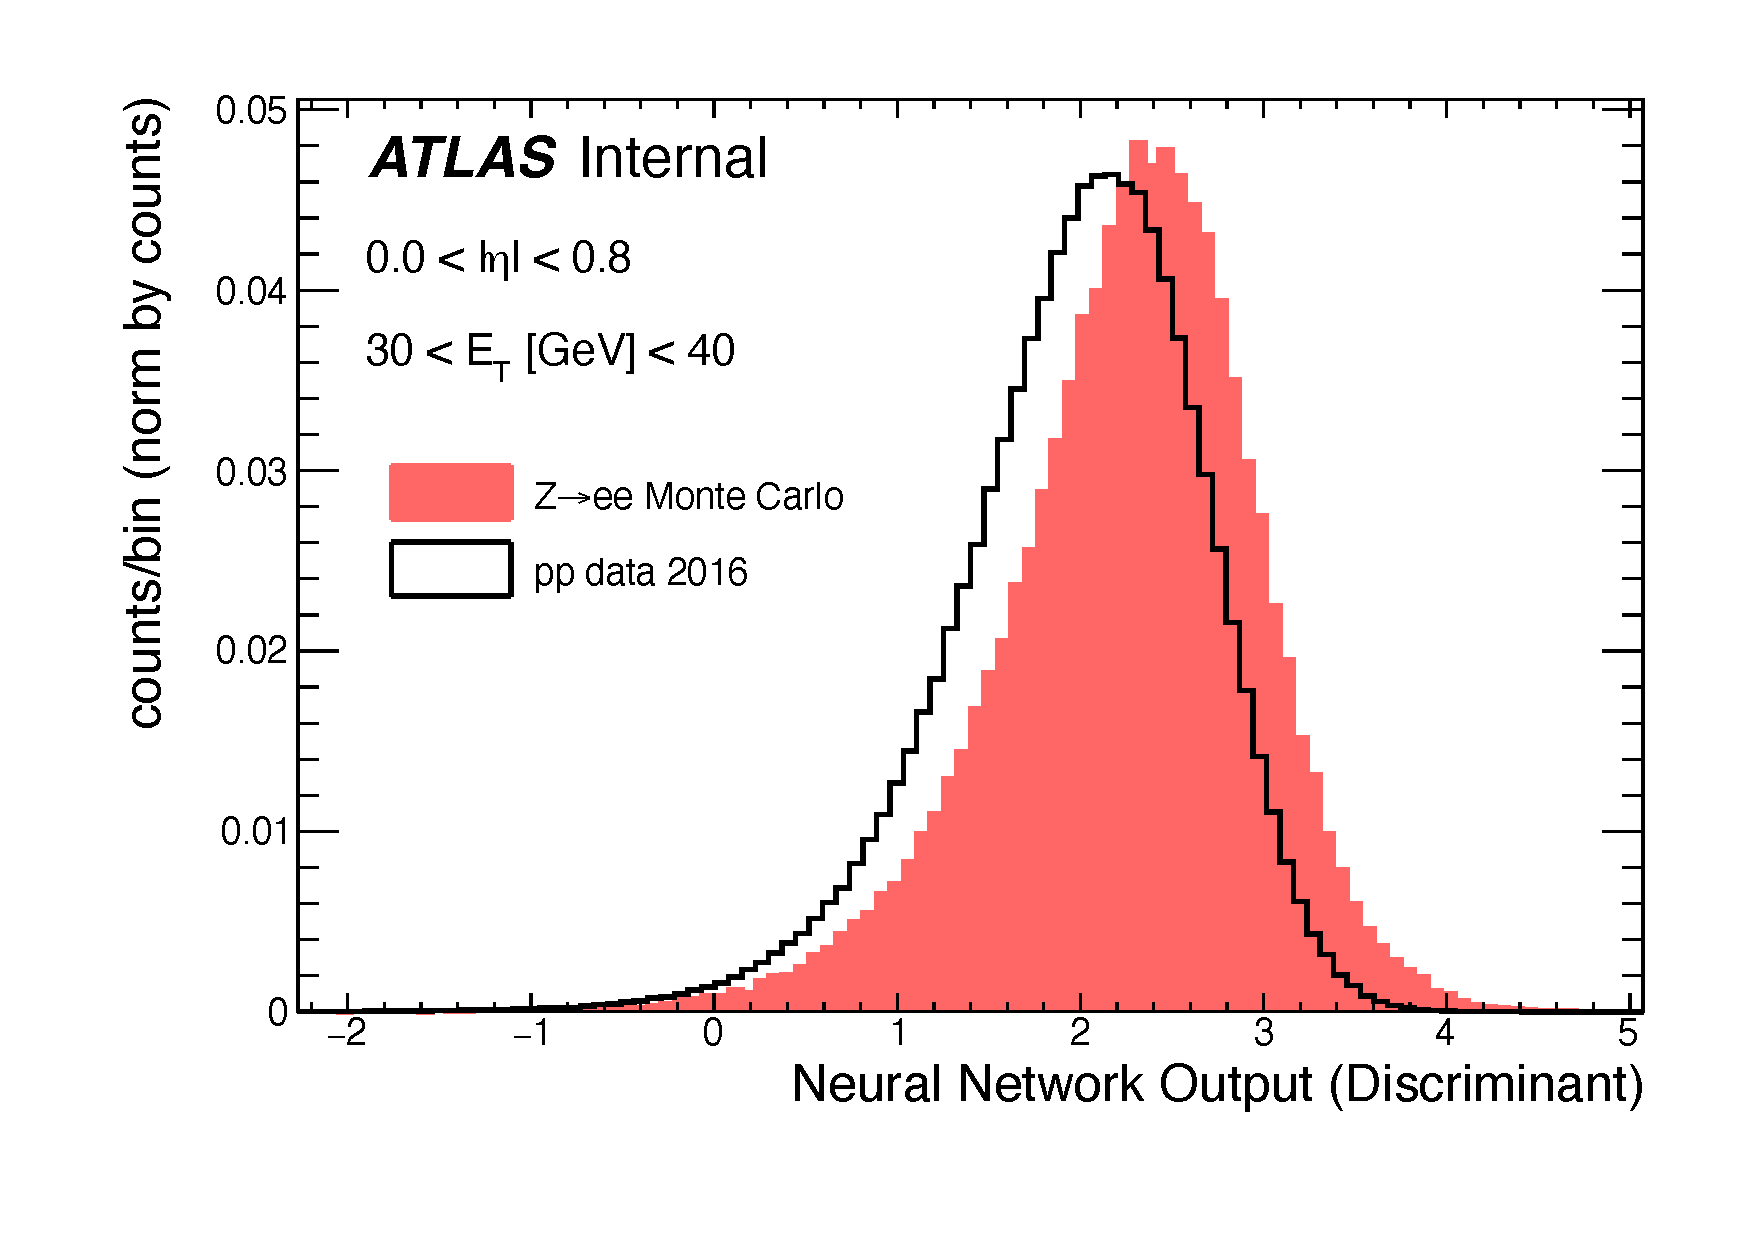
\includegraphics[width=0.7\textwidth]{sections/02_ringer/figures/nn_output_mc15_versus_data16_et2_eta0.pdf}
  \caption{Differences between simulation samples (red) from 2015 and collision data (black) obtained in 2016 for a region of the phase space.
  The comparison is made between the normalized distributions obtained in both cases for the output of the neural network (discriminant) generated for the samples present in the signal set within the selected region of the phase space. The shift on the discriminant generated by the neural network between simulation and collision data is caused by the differences of the simulation-data rings used as input of the model. }
  \label{fig:nn_mc15_vs_data16}
\end{figure}


Furthermore, it was observed
that the rings in the region $2.37<\abseta<2.47$ had particular profiles due to
the lack of strip cells in this region and demanded a specific discriminant requirement in order to keep signal efficiencies close to the cut-based triggers. In order to avoid retraining all models, it was decided to split the last $|\eta|$ region in two, from $1.37\rightarrow 2.5$ to $1.37\rightarrow2.37\rightarrow2.5$, and duplicate all models, for this region, to the new bin. Finally, the set used to operates in 2017 has a total of 25 MLP models. The set boundaries are defined by Table~\ref{tab:ensemble_regions}.



\begin{table}[htb]
\begin{center}
	{\small
	\begin{tabular}{cccc}
		\hline \hline
		\multicolumn{4}{c}{Model Adjust}                                                                 \\ \hline
		\multicolumn{2}{c|}{$E_T$ {[}GeV{]} Boundaries} & \multicolumn{2}{l}{$|\eta|$ Boundaries}        \\ \hline
		\multicolumn{2}{c|}{$15 \leq E_T < 20 $}        & \multicolumn{2}{l}{$0.00 \leq |\eta| < 0.80 $}   \\
		\multicolumn{2}{c|}{$20 \leq E_T < 30 $}        & \multicolumn{2}{l}{$0.80 \leq |\eta| < 1.37 $}  \\
		\multicolumn{2}{c|}{$30 \leq E_T < 40 $}        & \multicolumn{2}{l}{$1.37 \leq |\eta| < 1.54 $} \\
		\multicolumn{2}{c|}{$40 \leq E_T < 50 $}        & \multicolumn{2}{l}{$1.54 \leq |\eta| < 2.37 $} \\
		\multicolumn{2}{c|}{$50 \leq E_T < \infty $}    & \multicolumn{2}{l}{$2.37 \leq |\eta| < 2.47 $} \\ \hline \hline
	\end{tabular}
}
\end{center}
\caption{$E_T$ and $\eta$ boundaries used to create the set of neural networks.}
\label{tab:ensemble_regions}
\end{table}

On the other hand, the 2018 training procedure employed a single set structure for all working points and used the 2017 collision data, selected with  \Zee{} \tnp{} event selection, for training, as was the case for the derivation of offline and final \hlt likelihood models~\cite{aaboud2019electron}.
Most of the procedure was kept unchanged for 2018. In opposition to 2017, the developments for 2018 could benefit from collision data representing similar data taking conditions. To simplify the training strategy, the selection of three models for each training was abandoned, keeping only the \spmax{} model, as the previous approach was more complex without a clear return on trigger efficiency. 

Likewise, MLPs with 5 to 10 units in the hidden layer were tuned, as most models did not require more than 10 units in 2017. The training optimizer was changed to the \emph{Adam}~\cite{kingma2014adam}, instead RPROP, and the MLP model topology was modified to: a hidden layer with a fully connected neurons with a rectified linear units (RELU) as the activation function and an output layer with one neuron using the sigmoid as the activation function. With a larger time span for entering operation, specialized MLPs in the region where a change was detected in the ring profiles before 2017 operation between $2.37<\abseta<2.47$ was added, resulting in the operation of \SI{25}{MLPs}. Finally, the correction limit was set to $\avgmu{}=100$~collisions in other to extrapolate the operation of the models to a never reached pile-up level condition. 





